\documentclass[10pt,a4paper]{article}
\usepackage[utf8]{inputenc}
\usepackage{amsthm, amsmath, mathtools, amssymb}
\usepackage[intlimits]{esint}
\usepackage[left=1.5cm,right=1.5cm,top=2cm,bottom=2cm]{geometry}
\usepackage[colorlinks,linkcolor=blue,citecolor=blue,urlcolor=blue]{hyperref}
\usepackage{babel}
\usepackage{titlesec}
\usepackage{enumitem}
\usepackage{physics}

\newcommand{\NN}{\ensuremath{\mathbb{N}}} % set of natural numbers
\newcommand{\ZZ}{\ensuremath{\mathbb{Z}}} % set of integers
\newcommand{\QQ}{\ensuremath{\mathbb{Q}}} % set of rationals
\newcommand{\RR}{\ensuremath{\mathbb{R}}} % set of real numbers
\newcommand{\CC}{\ensuremath{\mathbb{C}}} % set of complex numbers
\newcommand{\KK}{\ensuremath{\mathbb{K}}} % a general field

%%%%%%%%%% Commands for Acronyms %%%%%%%%%%

\newcommand{\ICRF}{\ensuremath{\mathrm{ICRF}}}
\newcommand{\ITRF}{\ensuremath{\mathrm{ITRF}}}
\newcommand{\GMST}{\ensuremath{\mathrm{GMST}}}
\newcommand{\GAST}{\ensuremath{\mathrm{GAST}}}



\newcommand{\vf}[1]{\boldsymbol{\mathrm{#1}}} % math style for vectors and matrices and vector-values functions (previously it was \*vb{#1} but this does not apply to greek letters)
\newcommand{\ii}{\mathrm{i}} % imaginary unit
\renewcommand{\O}{\mathrm{O}} % big O-notation

\newtheorem{theorem}{Teorema}
\newtheorem{prop}{Proposició}
\theoremstyle{definition}
\newtheorem{definition}{Definició}
\DeclareDocumentCommand\derivative{ s o m g d() }{ 
  % Total derivative
  % s: star for \flatfrac flat derivative
  % o: optional n for nth derivative
  % m: mandatory (x in df/dx)
  % g: optional (f in df/dx)
  % d: long-form d/dx(...)
    \IfBooleanTF{#1}
    {\let\fractype\flatfrac}
    {\let\fractype\frac}
    \IfNoValueTF{#4}
    {
        \IfNoValueTF{#5}
        {\fractype{\diffd \IfNoValueTF{#2}{}{^{#2}}}{\diffd #3\IfNoValueTF{#2}{}{^{#2}}}}
        {\fractype{\diffd \IfNoValueTF{#2}{}{^{#2}}}{\diffd #3\IfNoValueTF{#2}{}{^{#2}}} \argopen(#5\argclose)}
    }
    {\fractype{\diffd \IfNoValueTF{#2}{}{^{#2}} #3}{\diffd #4\IfNoValueTF{#2}{}{^{#2}}}\IfValueT{#5}{(#5)}}
} % differential operator
\DeclareDocumentCommand\partialderivative{ s o m g d() }{ 
  % Total derivative
  % s: star for \flatfrac flat derivative
  % o: optional n for nth derivative
  % m: mandatory (x in df/dx)
  % g: optional (f in df/dx)
  % d: long-form d/dx(...)
  \IfBooleanTF{#1}
    {\let\fractype\flatfrac}
    {\let\fractype\frac}
    \IfNoValueTF{#4}{
      \IfNoValueTF{#5}
      {\fractype{\partial \IfNoValueTF{#2}{}{^{#2}}}{\partial #3\IfNoValueTF{#2}{}{^{#2}}}}
      {\fractype{\partial \IfNoValueTF{#2}{}{^{#2}}}{\partial #3\IfNoValueTF{#2}{}{^{#2}}} \argopen(#5\argclose)}
    }
    {\fractype{\partial \IfNoValueTF{#2}{}{^{#2}} #3}{\partial #4\IfNoValueTF{#2}{}{^{#2}}}\IfValueT{#5}{(#5)}}
} % partial differential operator


\renewcommand{\exp}[1]{\mathrm{e}^{#1}} % exponential function
\DeclareMathOperator*{\im}{Im}

\setlength{\parindent}{0pt}
\begin{document}
\section{Notes on transformations between systems of coordinates}
\subsection{Introduction}
The TLE data (mainly the \emph{inclination} $i$, the \emph{right ascension of the ascending node} $\Omega$, the \emph{eccentricity} $e$, the \emph{argument of the perigee} $\omega$, the \emph{mean anomaly} $M$ (angle of the body from the perigee if it was in a circular orbit imposing to have the same period, not to be confused with the \emph{true anomaly} $\nu$ nor with the \emph{eccentric anomaly} $E$ (same as $\nu$ but the angle is respect to an auxiliary circle)) and the mean motion $n=\frac{2\pi}{P}$ (the revolutions per day, which implies knowing the semi-major axis by the Kepler 3rd law: $\mu=a^3n^2$, $\mu=GM$)) is referred to the angles with respect to the equatorial plane at the J2000 epoch and we need to integrate the system in an almost-inertial Reference Frame, but we need the Geopotential coefficients (that depend on the latitude and longitude of the satellite). Thus we need to move the satellite to the ITRF frame and then back to the ICRF.

Thus, we need to know the position of the earth rotation axis as a function of time based on the J2000. Once got it, we will (at first) fix the axis for the sake of simplicity (as we are only integrating trajectories during a few days or weeks). There are 4 main influences that affect the position of the axis:

\begin{enumerate}
  \item The precession of the equinoxes:
        \begin{definition}
          The \emph{mean equinox} is the position of the equinox when solar precession alone is taken into account. The \emph{apparent equinox} is the actual equinox direction when both precession and nutation are included.
        \end{definition}
        \begin{figure}[ht]
          \centering
          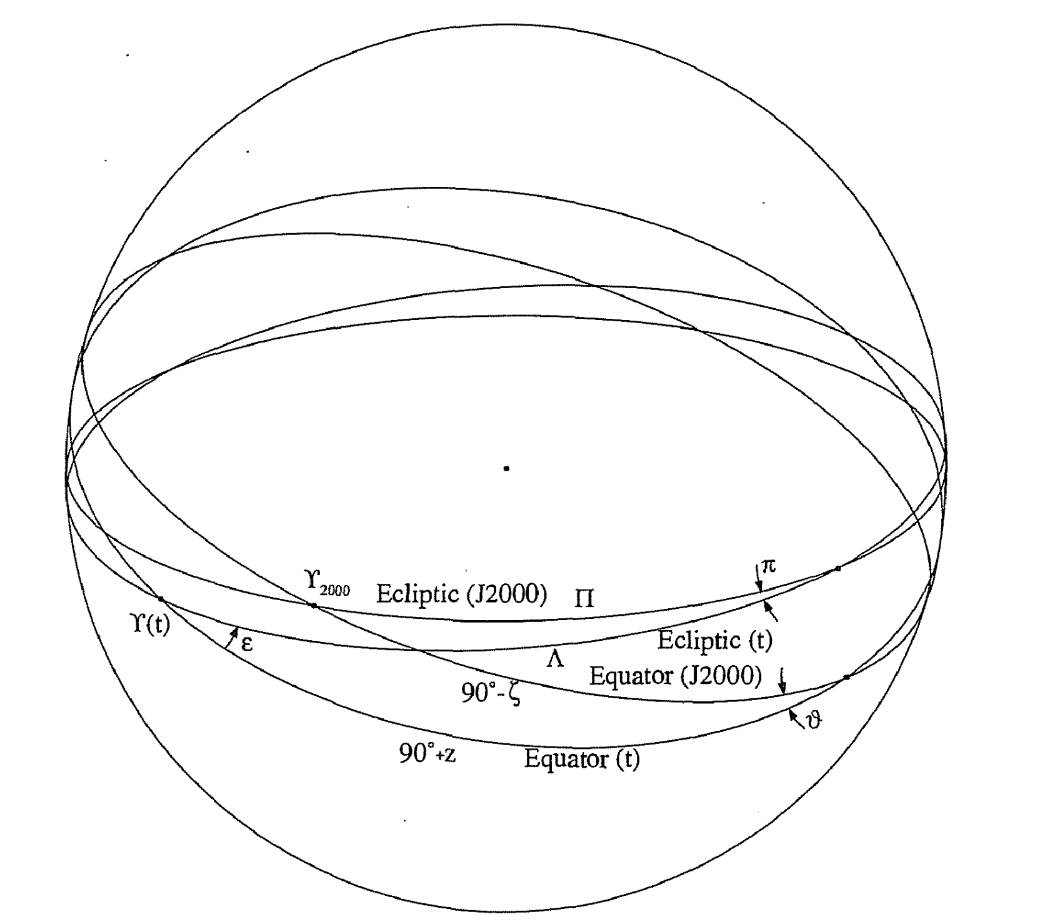
\includegraphics[width=0.5\textwidth]{Images/celestialSphereMonte.png}
          \caption{Ecliptic and equatorial plane in the J2000 frame and at some other epoch.}
        \end{figure}
        It's easy to see that if $\vf{P}$ is the rotation matrix that carries the mean Equator (J2000) to the mean Equator (T) and also the respective equinoxes $\Upsilon_{2000}$ and $\Upsilon_T$ we have that:
        $$\vf{r}_T=\vf{P}\vf{r}_{J2000}=\vf{R}_z(-90-z)\vf{R}_x(\theta)\vf{R}_z(90-\zeta)\vf{r}_{J2000}$$
        Which can be simplified to:
        $$\boxed{\vf{P}(T)=\vf{R}_z(-z)\vf{R}_y(\theta)\vf{R}_z(-\zeta)}$$
        where $T=\frac{JD-2451545}{365.25}$ are Julian centuries since J2000 TT. The dependence on the time of each of the angles is given in the Montenbruck.

        Here the elementary rotation matrices are:
        $$\vf{R}_x(\theta)=\begin{pmatrix}
            1 & 0           & 0          \\
            0 & \cos\theta  & \sin\theta \\
            0 & -\sin\theta & \cos\theta
          \end{pmatrix}\qquad\vf{R}_y(\theta)=\begin{pmatrix}
            \cos\theta & 0 & -\sin\theta \\
            0          & 1 & 0           \\
            \sin\theta & 0 & \cos\theta
          \end{pmatrix}\qquad\vf{R}_z(\theta)=\begin{pmatrix}
            \cos\theta  & \sin\theta & 0 \\
            -\sin\theta & \cos\theta & 0 \\
            0           & 0          & 1
          \end{pmatrix}$$
        (see Goldstein 1980)
  \item The nutation

        \begin{figure}[ht]
          \centering
          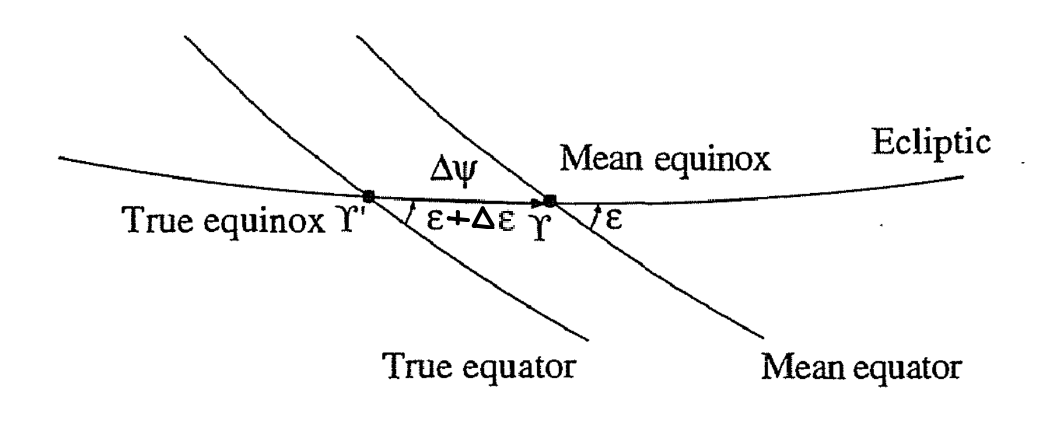
\includegraphics[width=0.5\textwidth]{Images/nutationMonte.png}
          \caption{Nutations change.}
        \end{figure}
        Due to the nutation changes, we need to carry the mean equator and mean equinox (at the epoch $t$) to the true ones (at the epoch $t$) with a matrix $\vf{N}$ equal to:
        $$\boxed{\vf{N}(T)=\vf{R}_x(-\varepsilon-\Delta\varepsilon)\vf{R}_z(-\Delta\psi)\vf{R}_x(\varepsilon)}$$
        The dependence on the time of each of the angles is given in the Montenbruck.
        % Note the IERS 1996 added a correction to the nutation quantities of several mili-arcseconds (see Montenbruck p.180 for further info).

  \item The Earth's rotation

        \begin{definition}
          The rotation about the CEP (\emph{Celestial Ephemeris Pole}) axis itself is described by the Greenwich Mean Sidereal Time (GMST) that measures the angle between the mean vernal equinox and the Greenwich Meridian. From Montenbruck p.181:

          \textit{The Celestial Ephemeris Pole differs slightly from the instantaneous rotation axis which was used in the earlier nutation theory of Woolard (1953). The adoption of the CEP is related to the fact that the rotation axis performs a predictable daily motion around the CEP under the action of Sun and Moon and is not, therefore, a proper reference pole for theoretical and observational reasons. On the Earth's surface the difference between both poles amounts to approximately 0.6 m.}
        \end{definition}
        \begin{figure}[ht]
          \centering
          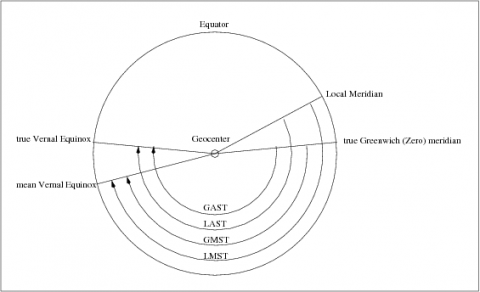
\includegraphics[width=0.5\textwidth]{Images/siderialtime.png}
          \caption{Siderial time}
        \end{figure}
        The rotation of the Earth is described by the GAST with the matrix:
        $$\boxed{\vf\Theta(T)=\vf{R}_z(\mathrm{GAST})}$$
        where:
        \begin{align*}
          \mathrm{GAST} & =\mathrm{GMST}+\alpha_E                         \\
          \mathrm{GMST} & =\mathrm{GMST}_0+1.0027379093\cdot \mathrm{UT1} \\
        \end{align*}
        where UT1 is the \emph{Universal time}. $\mathrm{GMST}_0$ is given in Montenbruck. The $\alpha_E$ is the difference between the hour angle of the true equinox of date and the mean equinox  of date, difference which is due to the nutation of earth and can be computed from:
        $$\alpha_E=\arctan(\vf{N}_{12}/\vf{N}_{11})\approx\Delta\psi\cos\varepsilon$$
  \item The polar motion

        The polar motion can be modelized by the matrix $$\vf{\Pi}(T)=\vf{R}_y(-x_p)\vf{R}_x(-y_p)$$
        where $x_p$ and $y_p$ are the polar motion coordinates. The polar motion is the displacement of the CEP pole with respect to the ITRF (\emph{International Terrestrial Reference Frame}) pole. The ITRF pole is the pole of the Earth's rotation axis. The values $x_p$ and $y_p$ are obtained from a least-squares fit to six years of past polar motion data.
        \begin{figure}[ht]
          \centering
          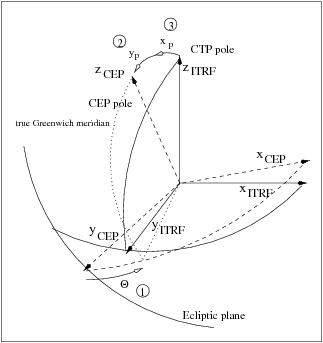
\includegraphics[width=0.5\textwidth]{Images/cepToITRF.png}
          \caption{CEP to ITRF transformation}
        \end{figure}
\end{enumerate}
So the general formula to pass from ICRF to ITRF is:
$$\vf{r}_\mathrm{ITRF}=\vf{\Pi}(t)\vf\Theta(t)\vf{N}(t)\vf{P}(t)\vf{r}_\mathrm{ICRF}$$
where $\vf{r}_\mathrm{ICRF}$ is the position vector of the object in the ICRF frame and $\vf{r}_\mathrm{ITRF}$ is the position vector of the object in the ITRF frame.

In order to compute the velocity and acceleration transformsations between those frames, if we consider consider the polar motion, nutation and precession matrices as constant, we have:
\begin{align*}
  \vf{v}_\mathrm{ITRF} & =\vf{\Pi}\dot{\vf\Theta}\vf{N}\vf{P}\vf{r}_\mathrm{ICRF}+\vf{\Pi}{\vf\Theta}\vf{N}\vf{P}\vf{v}_\mathrm{ICRF}                                                           \\
  \vf{a}_\mathrm{ITRF} & =\vf{\Pi}\ddot{\vf\Theta}\vf{N}\vf{P}\vf{r}_\mathrm{ICRF}+2\vf{\Pi}\dot{\vf\Theta}\vf{N}\vf{P}\vf{v}_\mathrm{ICRF}+\vf{\Pi}{\vf\Theta}\vf{N}\vf{P}\vf{a}_\mathrm{ICRF}
\end{align*}
where
\begin{align*}
  \dot{\vf\Theta} & =\dv{(\GAST)}{t}\begin{pmatrix}
                                      -\sin(\GAST) & \cos(\GAST)  & 0 \\
                                      -\cos(\GAST) & -\sin(\GAST) & 0 \\
                                      0            & 0            & 0
                                    \end{pmatrix} \\
\end{align*}
\subsubsection{Important note about JPL D400 series ephemerides}
They DO NOT use the J2000 frame. Instead, they use the ICRF (\emph{International Celestial Reference Frame}) whose origin is at the Barycenter of the Solar system and the axis are defined from quasars... From Montenbruck and Gill (2000) p.75 (also check p. 170 for further info):

\textit{ In the recent DE400 series all data are referred to the International Celestial Reference Frame (ICRF, cf. Sect. 5.2), which is realized through a catalog of radio sources. The difference between the dynamical J2000 reference frame and the ICRF is at a level of 0.01'', and determined with an accuracy of 0.003'' (Standish et al. 1995).}

From NASA:

\textit{ The realization of ICRF was made to coincide almost exactly with the J2000 frame. The difference is very small: a rotation of less than 0.1 arc second}

\subsubsection{Geocentric system}
On the orther hand, the earth-centered RF that will be using is the ITRF (\emph{International Terrestrial Reference Frame}) whose origin is at the Earth's center of mass, $x$-axis pointing to the 0-meridian and $z$-axis perpendicular to the equatorial plane.


\subsection{Transformations from orbital elements to Geocentric Equatorial Coordinates at epoch \texorpdfstring{$T$}{T}}

Idea: $$\mathrm{TLE}\to\vf{r}\text{ and }\vf{v}\text{ from a RF in the orbital plane}\to \text{Geocentric RF at epoch $T$}\to\text{Geocentric RF at epoch J2000}$$

Note: to pass from hight $H$ and latitude to coordinates in the ITRF, see Bate-Mueller-White p.98.


% Consider the planar reference frame ($\vf{P}$, $\vf{Q}$) based on the orbital plane of a satellite. Assume $\vf{P}$ points to the perigee and $\vf{Q}$ is such that the basis is positive. Let $\vf{W}$ be the normal vector of the plane. The position $\vf{r}$ and velocity $\vf{v}$ of the satellite in the $\vf{P}$, $\vf{Q}$ frame are given by:
% \begin{align}
%   \vf{r} & = \left(\frac{a(1-e^2)}{1+e\cos\nu}\right)\left(\cos\nu\vf{P}+\sin\nu\vf{Q}\right)        \\
%   \vf{v} & = \frac{\sqrt{\mu a}}{1+e\cos\nu}\left(-\sin\nu\vf{P}+\left(e+\cos\nu\right)\vf{Q}\right)
% \end{align}
% \begin{proof}
%   We have that:
%   \begin{equation}
%     \vf{r} = r\left(\cos\nu\vf{P}+\sin\nu\vf{Q}\right)
%   \end{equation}
% \end{proof}

Other things to consider:
\begin{enumerate}
  \item Check Vallado p.107 for the table of the TLEs.
\end{enumerate}
\end{document}
